%%%%%%%%%%%%%%%%%%%%%%%%%%%%%%%%%%%%%%%%%%%%%%%%%%%%%%%%%%%%%%%%%%
%%%%%%%% CPSC 66 FALL 2021  REPORT %%%%%%%%%%%%%%%%%%%%%%%%
%%%%%%%% This template is modified from ICML 2014 %%%%%%%%%%%%%%%%
%%%%%%%%%%%%%%%%%%%%%%%%%%%%%%%%%%%%%%%%%%%%%%%%%%%%%%%%%%%%%%%%%%

\documentclass{article}

%include any external packages here.  This is similar to loading a
%library in python or C++

% use Times
\usepackage{times}
% For figures
\usepackage{graphicx}
\usepackage{subfigure}

% For citations
\usepackage{natbib}

% For algorithms and pseudocode
\usepackage{algorithm}
\usepackage{algorithmic}

%Adds hyperlinks to your citations automatically
\usepackage{hyperref}

% Packages hyperref and algorithmic misbehave sometimes.  We can fix
% this with the following command.
\newcommand{\theHalgorithm}{\arabic{algorithm}}

\usepackage[accepted]{icml2014}


% If your title is long (below), use this command to also provide
% short version.  This will go on the top of every page
\icmltitlerunning{Final Report}

\begin{document}

\twocolumn[ %use two column if you need a text to span across the whole page
\icmltitle{ CPSC 66 Final Report: \\ % \\ force a new line
Multi-label Classification with K-Nearest Neighbor }

\icmlauthor{Branley Mmasi}{bmmasi@swarthmore.edu}
\icmlauthor{David Liu}{dliu1swarthmore.edu}

\vskip 0.3in
]

\begin{abstract}
Classification problems generally focus on classifying novel examples into a given class, however, real-life examples often belong to multiple classes, or none at all, a problem referred to as multi-label classification. In this paper, we follow Chiang et al.'s 2012 approach for this problem, using a modified K-Nearest Neighbor (kNN) algorithm to predict the EC-classes of various substrate molecules. Instead of traditional kNN, which considers a novel query's k neighbors equally, this modified approach ranks neighbors based on trustworthiness and weighs their labels accordingly. To measure overall performance, we used Hamming Loss as our evaluation metric. We then compared our results against a traditional kNN approach. For lower k's, we found that traditional kNN heavily outperforms modified kNN, but for larger k's, their overall performance begins to converge. However, with an overall Hamming Loss of 0.3, we recognize that our model alone is still likely unable to be used in any meaningful applications.


\end{abstract}

\section{Introduction}
\label{introduction}

Classification problems often focus on predicting a single class given a novel query, and numerous machine learning models, including kNN, decision trees, and logistic regression have been developed to solve these problems. However, real-life examples often contain more than one label, for instance, rice could be classified as a staple of both Chinese and Japanese cuisine. Or, as common in social media sites, images and posts can be tagged with multiple tags at once. 

If all labels were independent of each other, then one might simply approach a multi-label classification problem as multiple single-label classification problems, predicting each label separately. However, most of the time, that is not the case. In the case of foods for example, foods staple to Chinese cuisine will more often than not be found in Japanese cuisine compared to French cuisine. Tags in social media also appear together with some tags more than others. In that case, in developing a multi-label classification model, it is important to find and exploit correlations between labels\cite{chiang}.

In this paper, we follow Chiang et al.'s 2012 paper, modifying a traditional kNN model and apply it to multi-label classification. The 2012 paper proposes the training of a global ranking model based on neighbors' trustworthiness, then using a weighted voting strategy to predict the final label prediction of a query. 

However, because of time and knowledge constraints, we were unable to implement their ranking model, and we simplified their generalized pattern search weighting method into one that directly used the Hamming loss of a query's neighbors to generate the weights. 

\section{Methods}
\label{methods}

At a high level, our modified kNN approach first trains a Linear Regression model with its training data to predict the Hamming loss of k neighbors of each training point compared to its own label set. Then, for a novel query x, it predicts the Hamming loss of each of x's neighbors, and uses those Hamming losses to generate weights for the neighbors. Finally, we use those weights to predict the label set of x.

\begin{figure}[ht]
\vskip 0.2in
\begin{center}
\centerline{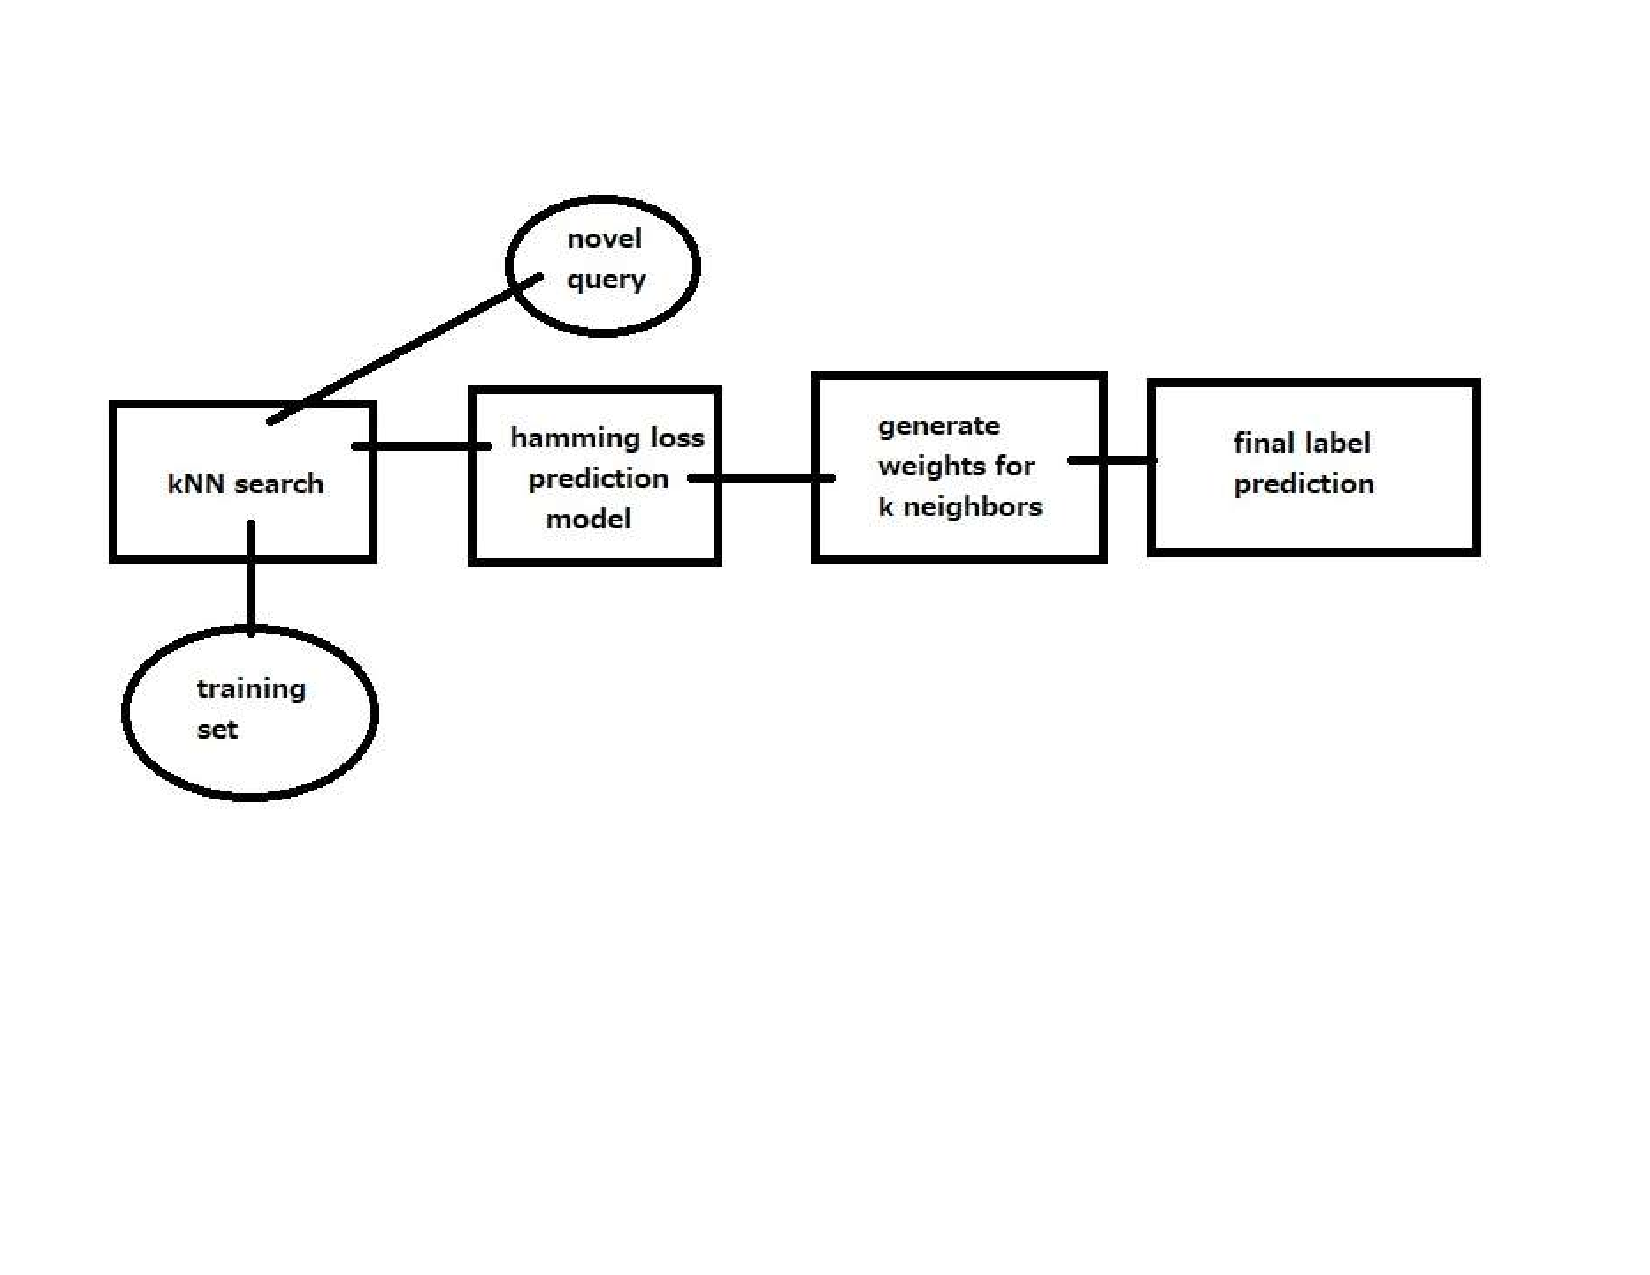
\includegraphics[width=\columnwidth]{diagram}}
\caption{Overall approach for modified kNN}
\label{icml-historical}
\end{center}
\vskip -0.2in
\end{figure}

\subsection{Training Data}

To create our Linear Regression model that predicts Hamming loss, we first find k neighbors of each point z in our training data. Next, for each neighbor k, we create a new point $q_i$ which contains:
\begin{itemize}
\item The feature distance between every feature of z and its neighbor
\item The Euclidean distance between z and its neighbor
\item The cosine distance between z and its neighbor
\end{itemize}

Next, we compute the Hamming loss between z and each of its neighbors. Hamming loss is simply the percentage of labels that is different between two label sets, defined as:

$HammingLoss(L1,L2) = |L1 \delta L2|/|L|$

Then, we use our results to train a Linear Regression model, where $q_i$ is the inputs, and the prediction is the Hamming loss. 

\begin{algorithm}
   \caption{Create Hamming loss Prediction Model}
   \label{alg:example}
\begin{algorithmic}
    \FOR{$T_i=1$ {\bfseries to} $T$}
    \FOR{$k=1$ {\bfseries to} $k$}
   \STATE q = (Feature Distances, Euclidean Distance, Cosine Distance)
   \STATE h = HammingLoss($T_i$,k)
   \STATE Q.append(q), H.append(h)
   \ENDFOR
    \ENDFOR
    \STATE MODEL = LinearRegression(Q,H)
\end{algorithmic}
\end{algorithm}

This is where Chiang et al. created their ranking model as opposed to a direct Hamming loss prediction model that we have here. As seen later in the paper, due to a lack of a ranking model, a novel query x in our algorithm will still use its initial k neighbors as opposed to a new set of ranked k neighbors. This significantly worsens our predictions, as we are then unable to choose the most trustworthy neighbors out of the entire set. Instead, we are forced to use x's k neighbors, and can only assign weights to try and compensate\yrcite{chiang}. 

\subsection{Generating Label Set of Novel Query}

For a new query x, we first find its k nearest neighbors, and generate q identically to the above methodology. Next, we use q to predict the Hamming loss of each of its neighbors. A lower Hamming loss means that a neighbor likely shares more labels with x, hence we assign it a higher weight. We went with a simple weighting system: 

$W = 1 - PredictedHammingLoss$

To predict the final label set of x, we produce an accumulated score for each label i, based on the weights of each of its neighbors:

$Label_i(x) = \sum_{j=1}^{k} w_j * Y_k,j / \sum_{j=1}^{k} w_j$ 

Where $Y_k,j$ is the ith label value of x's kth neighbor. The denominator is a normalization factor.

Here, we are restricting label values to be either 1 (presence of that label), or -1 (absence of that label).

We then assign x the label 1 if $Label_i(x) > 0$, else we assign it 0.

The final predicted label set will simply be the collection of all individual predicted labels.

Essentially, if most weighted neighbors have a positive label, then we also predict x's label to be positive, and vice versa\cite{chiang}.

\begin{algorithm}
   \caption{Predict Label Set of Novel Query}
   \label{alg:example}
\begin{algorithmic}

    \FOR{$k=1$ {\bfseries to} $k$}
   \STATE q = (Feature Distances, Euclidean Distance, Cosine Distance)
   \STATE W.append(1-MODEL.Predict(x,q))
   \ENDFOR
    \FOR {$i=1$ {\bfseries to} $labels$}
    \STATE RESULT.append($Label_i(x)$)
    \ENDFOR
\end{algorithmic}
\end{algorithm}

\section{Experiments and Results}
\label{results}

\subsection{Experimental Methodology}

We used a dataset containing data on substrate molecules, which all belong to multiple EC-Classes. EC-classes identify structural similarities between certain molecules, and as the dataset notes, this is particularly useful in drug discovery where enzymes will act upon substrates with similar structures as their substrates. In other words, if we are able to accurately identify which EC-classes the substrates belong to, we can predict the behavior of enzymes on other similar molecules.

The dataset contains 1039 molecules, each with 196 features, as well as a labelset identifying which EC-class(es) they belong to. The dataset notes that there is a high label imbalance, with the smallest label count being 1 and the highest label count being 248. This is actually something that we did not pay too much attention to during our design and implementation, and in hindsight, was something that likely affected our results\cite{enzyme}.

For preprocessing, since standard Linear Regression libraries cannot deal with NaN values, we had to decide whether to set them to a value or throw away the entire column altogether. Luckily, NaN values were restricted to a few columns, and most data points had NaN in those columns, so we were comfortable with just throwing away the columns. We also removed the CIDs column and normalized feature values to be between 0 and 1. Finally, we split the label set into an array of arrays of 1's and 0's. 

Due to time restrictions, we were unfortunately unable to perform any sort of cross-validation or repeated testing on our data. In large part, this is due to the fact that our kNN algorithm was not optimized for runtime, and one iteration of the training process took hours, especially with higher k's, which is something we should have anticipated, but we didn't really consider it during our implementation. kNN models become extremely expensive as they are scaled upwards, mainly because for each training point, the model must search n points k times. With a 60/40 train-test split for k=15, our model took over 2 hours to run. 

Instead, we opted to do a single 60-40 train-test split on our data and test multiple k's, then examine the results from that. We recognize that this method is by no means conclusive, and leaves a lot of ambiguity in our results. 

\subsection{Results}

\begin{table}[t]
\caption{Comparison of Hamming loss of traditional kNN and modified kNN}
\label{sample-table}
\vskip 0.15in
\begin{center}
\begin{small}
\begin{sc}
\begin{tabular}{lccr}
\hline
\abovespace\belowspace
k & Traditional & Modified \\
\hline
\abovespace
3    & 0.34 & 0.54 \\
5    & 0.31 & 0.58\\
7    & 0.31 & 0.60 \\
11    & 0.31 & 0.34 \\
15     & 0.29 & 0.33\\
25      & 0.28 & 0.28 \\
\belowspace
\end{tabular}
\end{sc}
\end{small}
\end{center}
\vskip -0.1in
\end{table}

We used Hamming loss as our evaluation metric for overall performance of our model. While there exists other performances metrics, we followed Chiang et al.'s paper in using Hamming loss, and in general it is simple to calculate and an effective measuring tool. We then compared these results to a baseline, traditional kNN \yrcite{chiang}. To find average Hamming loss, we use:

$AverageHammingLoss = (1/|TestSet|) * \sum_{j=1}^{TestSet} HammingLoss(j,x) $

Our baseline kNN simply finds the k nearest neighbors of a novel query, then has the neighbors vote on each of the labels, which will then output the final label set. Despite k's ranging from 3 to 35, we found that traditional kNN performs very similarly in all situations, with an overall Hamming loss of 0.30.

Meanwhile, with our modified model, we found that our modified kNN actually does very poorly with small k's, getting about half the labels incorrect every time, which is no better than flipping a coin. Meanwhile, for higher k's greater than 10, our modified model begins to perform on par with traditional kNN, though still only at around a 0.3 Hamming loss.

\section{Discussion}
\label{discussion}

Without further testing, it is a bit tricky to determine why we obtained the results we did. One hypothesis for our model's performance could be attributed to the fact that it is much more complex than traditional kNN, meaning that it requires a higher k to have meaningful results. Compared to kNN, our modified kNN uses feature distances, euclidean distance, and cosine distance to create the model to predict weights. However, if the k is not high enough, then the model might potentially not have enough data to make accurate predictions, hence giving inaccurate weights. This pattern could explain why larger k's are preferred for modified kNN. Chiang et al.'s paper use a baseline of k=10, which somewhat reflects this hypothesis. 

We are not entirely sure why kNN performed just as well as our model, if not better. The simplest answer could be that directly predicting Hamming loss of k neighbors is not a very effective measure of weights, which we also believe to be the most probable reason. Another possibility could lie in our dataset - compared to Chiang et al.'s datasets which mostly had 10-40 labels, our dataset only had 6, as well as fewer examples. In other words, perhaps our dataset was too small and simple for a complex model to be very effective in predicting its labels. 

Comparing our results to Chiang et al.'s paper, their model consistently scored a Hamming loss of between 0.1 and 0.2 across numerous datasets, occasionally reaching close to 0 \yrcite{chiang}. As expected, a reranking of neighbors is a crucial step that allows the model to predict the neighbors which have the closest labels matching the a query point, which dramatically improves results.

\section{Conclusions}
\label{conclusion}

\subsection{Limitations}

In this paper, we implemented a modified kNN algorithm to tackle the multi-label classification problem. Due to limited time for testing, our results were not fully tested, but it is clear that our approach lacks the ability to predict labels any better than a regular kNN model naively voting for each label.

Our biggest limitation was the fact that we did not know anything about ranking models, and that following a paper centered around a ranking algorithm proved too difficult for us to fully understand and implement in the time we had. Another limitation, as discussed, was the fact that our algorithm was very expensive time-wise to run, meaning we were limited in the training and testing of our model.

\subsection{Future Research}

Though we did not perform any conclusive testing on the performance of our model, it is likely safe to say that our model is not a good one. If we had more time and knowledge, we would have liked to implement a ranking algorithm for our neighbors, which will likely prove very effective. 

\section*{Acknowledgments}

Dr. Ben Mitchell whom we consulted on literally everything 

% In the unusual situation where you want a paper to appear in the
% references without citing it in the main text, use \nocite

\bibliography{references}
\bibliographystyle{icml2014}

\end{document}


% This document was modified from the file originally made available by
% Pat Langley and Andrea Danyluk for ICML-2K. This version was
% created by Lise Getoor and Tobias Scheffer, it was slightly modified
% from the 2010 version by Thorsten Joachims & Johannes Fuernkranz,
% slightly modified from the 2009 version by Kiri Wagstaff and
% Sam Roweis's 2008 version, which is slightly modified from
% Prasad Tadepalli's 2007 version which is a lightly
% changed version of the previous year's version by Andrew Moore,
% which was in turn edited from those of Kristian Kersting and
% Codrina Lauth. Alex Smola contributed to the algorithmic style files.
